\input{configuration}

\title{Lecture 7 --- Security }

\author{Jeff Zarnett \\ \small \texttt{jzarnett@uwaterloo.ca}}
\institute{Department of Electrical and Computer Engineering \\
  University of Waterloo}
\date{\today}


\begin{document}

\begin{frame}
  \titlepage

 \end{frame}



\begin{frame}
\frametitle{Security, Report to the Bridge}


In a lot of books, and even in my original plan for how the lectures would be carried out, security was left to the end. 

\begin{center}
	
\includegraphics[width=0.3\textwidth]{images/worf.jpg}
\end{center}

Security is something you want to bake into your product and something you want to have in your mind when you are designing it. 

 \end{frame}


\begin{frame}
\frametitle{Terminology}

An \alert{attacker} is a malicious user who is trying to damage or exploit the system. 

A \alert{countermeasure} is some action or process we can take or implement to defend against attacks. 

\end{frame}


\begin{frame}
\frametitle{Security Policies}

In this lecture we will not go into the legal or ethical issues related to security.

We also will not discuss security policies that are designed by organizations to tell you what keeps the system secure. 

We will focus on how access is controlled in the database, and specifically about the SQL Injection attack. 


\end{frame}


\begin{frame}
\frametitle{Sensitive Data}

Databases contain a lot of data and some of it might be sensitive. 

It might be that it is personal information, such as medical history of a patient or an employee's home address.

\begin{center}
	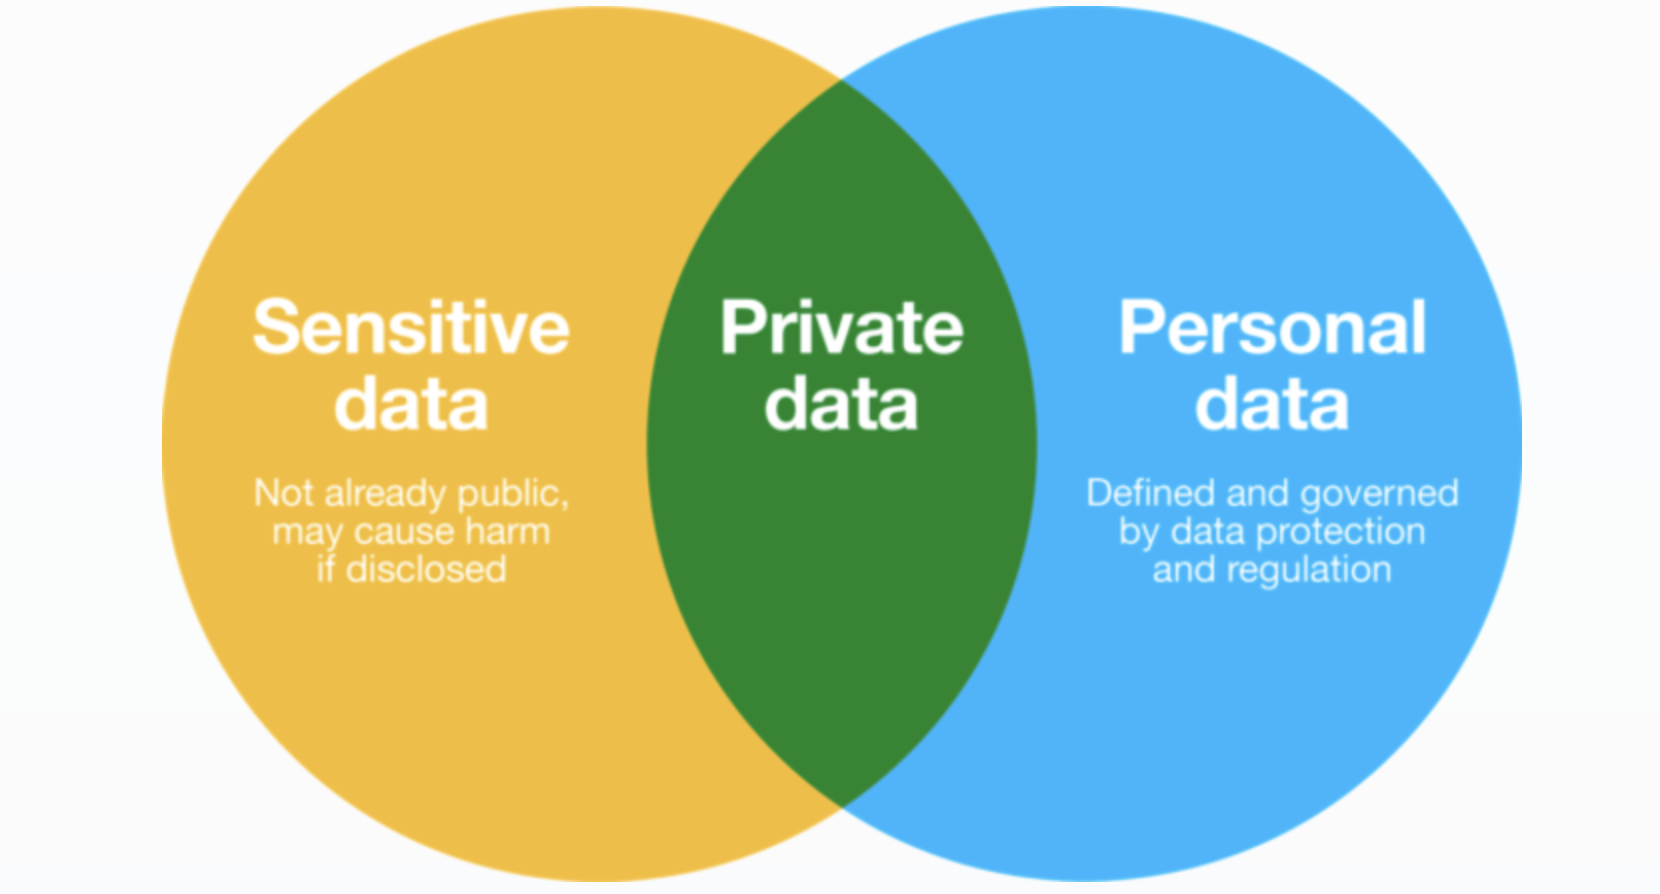
\includegraphics[width=0.7\textwidth]{images/private-data.png}
\end{center}

\end{frame}


\begin{frame}
\frametitle{Sensitive Data}


It could also be that it comes from a sensitive source. 

The sensitive data might not be the entire tuple; it might just be a particular attribute  such as Social Security Number or salary.


\end{frame}


\begin{frame}
\frametitle{Sensitive Data}

Regardless of why some data is sensitive, database administrators must see to it that the security policies are enforced. 

Ensure sensitive data is protected, but also that data is not corrupted and that access to any data is limited to those who should have access. 

\end{frame}


\begin{frame}
\frametitle{Sensitive Data}

Security policies do have some tradeoff with usability.

You most certainly do NOT want to find your company's name on TV having to report a data breach in which user personal data was stolen.

\begin{center}
	
\includegraphics[width=0.4\textwidth]{images/data-breach.png}
\end{center}

\end{frame}



\begin{frame}
\frametitle{Access Control}

We will talk about access control: what users have access to what in the DB. 

If this is configured correctly, then a lot of the security (although not all) is handled by the database server. 

But like seatbelts, access control doesn't work if you don't use it.

\end{frame}



\begin{frame}
\frametitle{The DBA}

It is the job of the database administrator to control accounts and privileges. 

This is analogous to the administrator or root or superuser account in operating systems, in that they have permissions to do everything and anything... 

But it is not good practice to log in using that account... 

\end{frame}


\begin{frame}
\frametitle{Storing Internally}

\begin{center}
	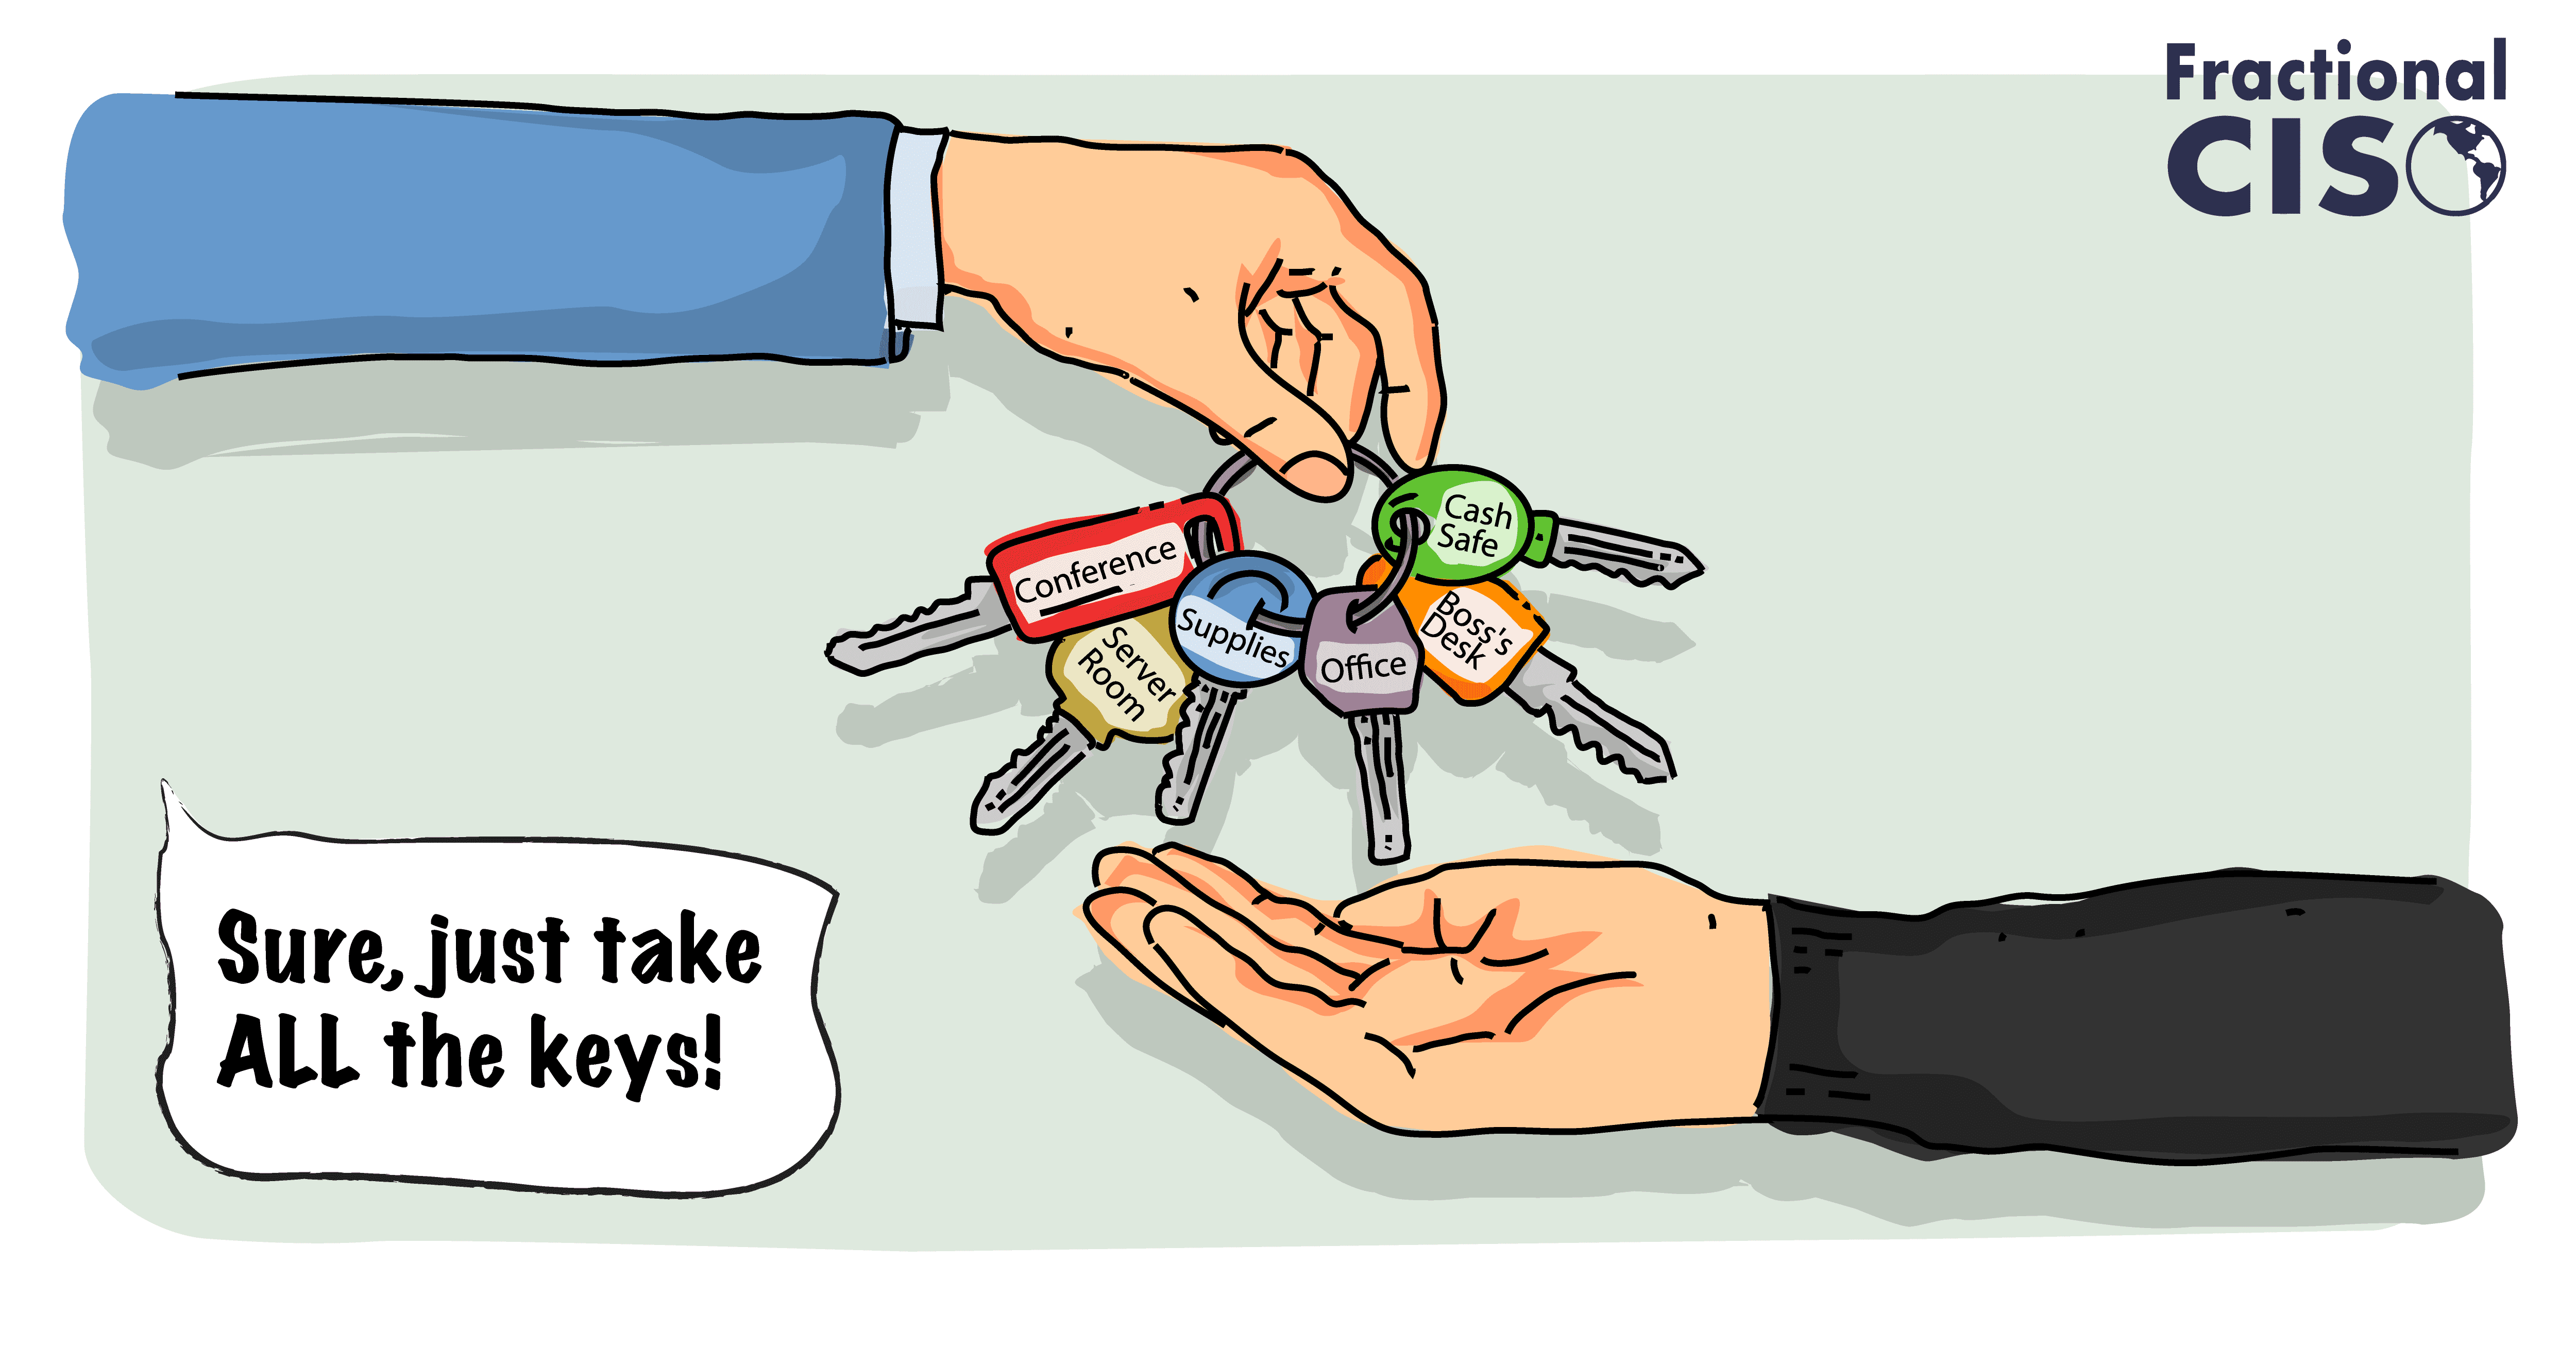
\includegraphics[width=0.7\textwidth]{images/least-privilege.png}
\end{center}

It is better to create limited accounts and assign only the exact privileges needed to those accounts...

\end{frame}



\begin{frame}
\frametitle{Username and Password}

Database systems have accounts and user accounts have passwords. 

Users are expected to log in with names and passwords when access is needed. 

The user name and password will be checked by the database server and if they match, the user is granted access. Otherwise, access denied.


\end{frame}


\begin{frame}
\frametitle{Storing Internally}

The database itself will likely use some tables internally.

When accounts and permissions are created they are recorded in the database's internal tables. 

After all, the data could be organized using the toolset we already have... relational database tables. 



\end{frame}



\begin{frame}
\frametitle{Audit Trail}

When a database user has successfully logged in, they have a \alert{login session}.

The session is associated with all of the interactions that user does while logged in. 

\begin{center}
	
\includegraphics[width=0.5\textwidth]{images/notes.jpg}
\end{center}

\end{frame}



\begin{frame}
\frametitle{Audit Trail}

This can be used to track who has logged in and who made what changes so that administrators can see the history in case something has gone wrong. 

If any malfeasance is suspected, database administrators can audit the logs (look through them) and determine what happened.  


\end{frame}



\begin{frame}
\frametitle{Granting Permissions}

Privileges can be given out at the account level: and includes the create schema, create table, create view, alter, drop, modify, select... 

Users are created with syntax like: \texttt{CREATE USER 'exampleuser'@'server' IDENTIFIED BY 'weakpassword';} 

To delete a user, \texttt{DROP USER exampleuser;}. 
 
To change a user's password, \texttt{SET PASSWORD FOR 'exampleuser'@'server' = PASSWORD ('CorrectHorseBatteryStaple');}

\end{frame}



\begin{frame}
\frametitle{Granting Permissions}

The next level is at relation level. 

Relations typically have an owner, usually the account used when the relation was created. 

It is likely that when a database schema is being created for the first time, an administrator account (eg root) is doing the creating. 

And the owner can allow other users to access it by \alert{granting} them access.


\end{frame}



\begin{frame}
\frametitle{Granting Permissions}

The keyword for this is \texttt{GRANT} and we'll soon see how it all works. 

The following privileges may be granted:

\begin{itemize}
	\item \textbf{Select}
	\item \textbf{Modification}
	\item \textbf{Reference Privilege}
\end{itemize}

Obviously, if privileges can be granted, they should also be able to be revoked. For that purpose, of course, there is the \texttt{REVOKE} command. 

\end{frame}



\begin{frame}
\frametitle{Using Grant}

Our basic syntax is: \textbf{GRANT} <privilege list> ON <relation> TO <user list>; 

So if we want to allow selection for user Alice on the table for books, it is \texttt{GRANT SELECT ON books TO alice;}.

 We can be as specific as we want to be: \texttt{GRANT UPDATE books( price ) TO bob, charlie, donna;} 
 
\end{frame}



\begin{frame}
\frametitle{Using Grant}
 
If we didn't specify any particular attributes, it would be possible to update all attributes of the relation. 

We can also grant \texttt{ALL} to give all privileges. 

\end{frame}



\begin{frame}
\frametitle{The Public}

It is possible to grant permissions to a special username, ``public'', which assigns the permission to all current and future users of the system. 

I really recommend against this sort of broad authorization. 

It goes against the idea of the principle of least privilege: user accounts should have only the privileges they need and nothing more.

\end{frame}



\begin{frame}
\frametitle{Revocation}

The revocation basic syntax is as follows: \textbf{REVOKE} <privilege list> ON <relation> FROM <user list>.

So if we no longer want to allow selection for user Alice on the table for books, it is \texttt{REVOKE SELECT ON books FROM alice;}. 

\begin{center}
	
\includegraphics[width=0.4\textwidth]{images/revoked.jpg}
\end{center}

\end{frame}



\begin{frame}
\frametitle{Why Reference?}

Are  you wondering why we might ever want to grant the reference privilege?

\begin{center}
	
\includegraphics[width=0.5\textwidth]{images/cap-reference.png}
\end{center}

\end{frame}



\begin{frame}
\frametitle{Why Reference?}


Foreign key constraints restrict deletion and update operations on the referenced relation. 

If someone creates a table $B$ referencing another $A$, then an attempt to delete an element from $A$ may fail due to the foreign key constraint added by $B$. 

Thus, it is sensible to have the references privilege, since the ability to add a foreign key restricts future activity by other users.

\end{frame}



\begin{frame}
\frametitle{Logging in as Root}

It is easy to just ignore all this and allow all your users to have all permissions, but this is dangerous. 

In particular, you might not want to allow developers this access either. 

Manual changes to the database should probably be done via some sort of double-check system.


\end{frame}



\begin{frame}
\frametitle{Roles}

Giving out permissions individually to users might be rather tedious. 

Every time a new user is added it might be necessary to run hundreds of grant statements to that new user for each table.

To manage the complexity, we might want to use \alert{roles}. 

\end{frame}

\begin{frame}
\frametitle{Roles}

\begin{center}
	
\includegraphics[width=0.7\textwidth]{images/role-model.jpg}
\end{center}


\end{frame}



\begin{frame}
\frametitle{RBAC}

In Role-Based Access Control (RBAC), a set of roles is created, users are assigned roles, and access is granted or denied based on the role(s) a user has or lacks.

Thus, assigning rights to users is done by assigning roles to users. 

A user can have more than one role, but must have at least one.

An advantage this has over direct management of permission granting is that assignment is simpler.

\end{frame}



\begin{frame}
\frametitle{Roles in SQL}

Roles are created very simply in SQL: \texttt{CREATE ROLE accounting;} would create the role of accounting but it would not have any permissions. 

Then, we can grant permissions to this role as if it was a user: \texttt{GRANT SELECT ON payroll TO accounting;} would do the job. 

But then you need to give some users the role: \texttt{GRANT accounting TO leslie;}. 

Now Leslie will have all the privileges that are granted to the accounting role, including ones added to the role after it has been granted to Leslie. 


\end{frame}


\begin{frame}
\frametitle{Role Relations}

There can also be relations between roles: doctors might be able to do all the things a nurse can do. 

Rather than have extra permissions assigned everywhere, the system can be set up so the doctor role \textit{subsumes} the nurse role.

The doctor role has all the rights of the nurse role, and may have others. 

To do that, grant one role to the other: \texttt{GRANT nurse TO doctor;}


\end{frame}



\begin{frame}
\frametitle{Delegation}

It is also possible to delegate -- pass the authorization on to others -- if the permission for that is also granted. 

In the examples we have seen so far, the privileges cannot be granted by the recipient to any other users. 

If, however, we added the \texttt{WITH GRANT OPTION} at the end of the \texttt{GRANT} command, it means that the recipient may then grant that permission.

Alice would grant to Joe by issuing a grant command herself.

\end{frame}



\begin{frame}
\frametitle{Authorization Graph}
The database server will want to keep track of what permissions have been granted to which users and by whom.

\begin{center}
\includegraphics[width=0.35\textwidth]{images/auth-graph}
\end{center}

\end{frame}


\begin{frame}
\frametitle{Authorization Graph}

The graph can be checked for the existence of privileges. 

A user $U$ has a privilege $p$ if and only if there exists some path from the root (DBA account or root user) to $U$ (however many steps that takes). 

This is probably inefficient, as searching the tree on every transaction to see if the user doing the command has permission to do it is likely to take too long. 


\end{frame}



\begin{frame}
\frametitle{Authorization Graph}

What the graph is actually for is revocation. 

If in the diagram, $U_{1}$ has the permission revoked by the DBA, the permission that $U_{1}$ has granted to $U_{4}$ and $U_{5}$ will be revoked as well. 

This, in a practical sense, has no impact on $U_{5}$ because the permission has also been granted to $U_{5}$ by $U_{2}$, but $U_{4}$ can no longer perform the operation.


\end{frame}



\begin{frame}
\frametitle{Circular Argument is Circular}

You might think that you can trick the database! 

If $U_{8}$ grants the permission to $U_{9}$ and then $U_{9}$ grants it to $U_{8}$, if the database administrator revokes the permission grant to $U_{8}$, what happens? 

If we just used reference-counting, we would see that these users both have the permissions. 

But in constructing the graph we would see the problem immediately.

\end{frame}



\begin{frame}
\frametitle{Cascading Revocation}

There is the possibility to modify the revoke command to prevent cascading revocation; in that case just put \texttt{RESTRICT} at the end of the statement. 

If that is the case, then if the permission has been granted to anyone else, the revocation will not happen and the system will return an error.

The opposite of that is the \texttt{CASCADE} keyword, but it's unnecessary to use it because it is the default behaviour.

\end{frame}




\begin{frame}
\frametitle{Granting from a Role}

Sometimes we want to grant permission not from the current use but from a particular role.

 If that is the case, then add \texttt{GRANTED BY CURRENT\_ROLE} to the grant statement. 

Allowing users to grant roles is, in my opinion, fairly dangerous...

\end{frame}



\begin{frame}
\frametitle{SQL Injection}


\begin{center}
\includegraphics[width=0.95\textwidth]{images/exploits_of_a_mom}
\end{center}

\end{frame}



\begin{frame}
\frametitle{SQL Injection}

There are a few categories of things that can be accomplished by SQL injection:

\begin{itemize}
	\item \textbf{SQL Manipulation}
	\item \textbf{Code Injection}
	\item \textbf{Function Call Injection}
\end{itemize}

\end{frame}

\begin{frame}
\frametitle{SQL Injection}

And what can you do with this sort of access?
\begin{itemize}
	\item Execute arbitrary commands on the database (as we have seen).
	\item Determine what type of database is in the backend so we can see what is vulnerable.
	\item Denial of service attacks.
	\end{itemize}

\end{frame}


\begin{frame}
\frametitle{SQL Injection}

And what can you do with this sort of access?
\begin{itemize}

	\item Skip authentication (as above).
	\item Learn more about the internal structure of the application (mostly because error pages are very verbose).
	\item Privilege escalation -- gaining access to things that you should not be able to access.
\end{itemize}

\end{frame}



\begin{frame}
\frametitle{Avoiding SQL Injection}

In general the solutions are pretty well understood: user input should be filtered (sanitized) and not allowed to be put directly into the queries. 

This alone might not be enough, and it is better to bind the user input to parameters rather than dynamically building query strings. 

In this course we don't talk about how to write an application program that interacts with the database (we just tell the database what we want). 


\end{frame}



\begin{frame}
\frametitle{Encryption}

As another small note, data encryption is another way to protect your data. 

Sensitive data, such as passwords, must always be encrypted in the database. 

It should be encrypted with a one way hash function. 

\end{frame}



\begin{frame}
\frametitle{Encryption}

A security breach means that the passwords of your users will be leaked.

\begin{center}
	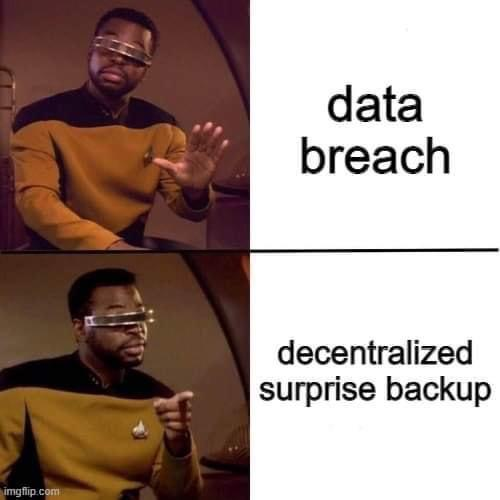
\includegraphics[width=0.4\textwidth]{images/dataleak.jpg}
\end{center}

Users re-use passwords between sites, so if someone's password on your service is leaked, it could very easily be someone's online banking password...


\end{frame}



\begin{frame}
\frametitle{Encryption Keys}
With that in mind, encryption keys should also not be stored in the database either... That would make it too easy for attackers! 

Or, if they are stored in the database, they can be stored encrypted. 


\end{frame}



\begin{frame}
\frametitle{Encryption Keys}

The standard sort of solution to this is to encrypt the key with the user's password. 

You don't want to see your company named and shamed on the news as having leaked the personal data of your users, do you?


\end{frame}

\end{document}

